\chapter{Words and Their Meanings}
\label{ch:words}

The pattern \code{11111111} can be read as 255, as -1, as eight Boolean
values, as a mask, or as one byte of an instruction. The pattern does not
confess which reading is intended. The operation or convention supplies it.

That distinction is the first foundation of instruction semantics. A register
stores a fixed number of bits. An operation supplies a reading and a rule for
producing another fixed pattern. We begin with the finite set on which all
those rules act.

\begin{figure}[htbp]
\centering
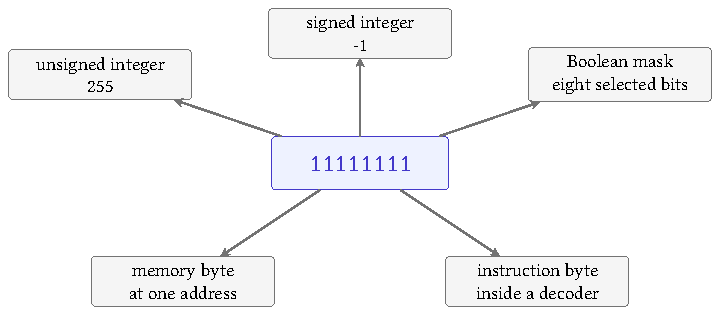
\includegraphics[width=0.92\textwidth]{figures/word-readings}
\caption{A stored pattern acquires a meaning only through a declared reading
or use. The arrows are interpretations, not changes to the eight bits.}
\figalt{The bits 11111111 point to unsigned 255, signed -1, a mask, a memory byte, and an instruction byte.}
\label{fig:word-readings}
\end{figure}

Figure~\ref{fig:word-readings} warns against a common shortcut. We may say
that a register ``contains -1'' when the signed reading is already clear. The
machine stores the pattern. The signed operation, comparison, conversion, or
printing convention supplies the -1. This distinction may feel fussy on one
byte. It becomes decisive when two instructions preserve the same bits but
give them different roles.

\subsection*{Positional notation made rules reusable}

A positional numeral assigns a weight to each place. In decimal, those
weights are powers of ten. In binary, they are powers of two. The gain is not
merely a shorter alphabet. One small collection of carrying and place-value
rules works at every position, so a finite procedure can act on numerals much
longer than the examples used to teach it.

Mechanical and electronic computers inherited that advantage. A circuit can
store two stable alternatives and combine them with Boolean operations. A
register groups a fixed number of those positions. The instruction set then
defines what operations may do to the group: add it, shift it, compare it,
split it into bytes, or treat it as an address.

Binary storage did not remove interpretation. It multiplied the useful
interpretations of one pattern. The same positions can support unsigned
arithmetic, two's-complement arithmetic, logical masks, encodings, and pieces
of larger structures. Modern verification must therefore bind the pattern to
the intended width and operation before it can establish a claim.

\begin{archive}[title={Place value is already an algorithmic idea}]
The written digits are finite data. A rule for their weights tells us how to
interpret every numeral of the admitted length. Machine words keep that
compact bargain and add a fixed boundary: beyond the highest position, the
operation must say what happens.
\end{archive}

\section{Writing patterns without losing the width}

Binary notation writes one symbol for every bit, which makes bit positions
visible and long words tiresome. Hexadecimal notation groups four bits into
one digit. The digits 0 through 9 keep their usual values; A through F stand
for 10 through 15. Thus
\[
  \mathtt{1111}=\mathtt{0xf}, \qquad
  \mathtt{1010\,0110}=\mathtt{0xa6}.
\]
The prefix \code{0x} tells us that the following digits are hexadecimal. It
does not tell us the width. The written numeral \code{0xff} may be an 8-bit
word, the low byte of a 32-bit word, or an integer literal that an assembler
will later fit into an instruction field.

\begin{keyidea}[title={A value is not yet a width}]
The numeral 255 names a mathematical integer. A word names an element of a
fixed finite set. Before applying a machine operation, state the width and the
rule that maps the numeral into that set.
\end{keyidea}

Leading zeroes carry this missing information when the context has not
already fixed it. The patterns \code{1111} and \code{00001111} have the same
unsigned reading, but they are different-width words. They offer different
high bits, different wraparound points, and different results under a
width-sensitive operation such as bitwise not.

\section{A finite circle}

Begin with a four-bit counter. It visits the patterns for 0 through 15. Add one
to 15 and the counter returns to 0 because there is no fifth bit in which to
store 16. This return to the start of a fixed-width range is
\keyterm{wraparound}. Add two to 15 and the counter stops at 1.

\begin{definition}[title={A0 word}]
For \(w \geq 1\), a \keyterm{word of width \(w\)} is a residue modulo
\(2^w\). We use the natural representatives
\(0,1,\ldots,2^w-1\). Addition, subtraction, and multiplication take the
ordinary integer result and keep its remainder modulo \(2^w\).
\end{definition}

Object \obj{A0.def.word} records this carrier and its readings. The quotient
notation says that integers differing by a multiple of \(2^w\) represent the
same stored word. At width four, 16 and 0 therefore represent the same word,
as do 17 and 1.

The reader proof of wraparound follows from division with remainder. For any
width-four word \(x\), ordinary addition gives \(x+1\). If \(x<15\), that
number already lies between 1 and 15, so taking the remainder changes nothing.
If \(x=15\), then
\(x+1=16=1\mathbin{\cdot}16+0\), whose remainder after division by 16 is 0.
The apparent exceptional case is simply the boundary of the finite carrier.

\begin{figure}[htbp]
\centering
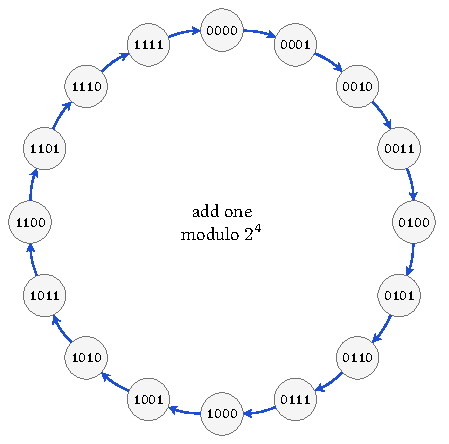
\includegraphics[width=0.52\textwidth]{figures/word-circle-four}
\caption{Addition by one visits every width-four word and returns to zero
after \code{1111}. The circular layout shows the modular rule; it is not a
picture of storage or time.}
\figalt{Sixteen four-bit words form a cycle under addition by one modulo 16.}
\label{fig:word-circle}
\end{figure}

The cycle in Figure~\ref{fig:word-circle} gives the right shape but not the
definition. A diagram might suggest that the counter physically travels
around a ring. It does not. The remainder operation supplies a successor for
each of the sixteen words, including the edge case \code{1111}. The circle is
useful because the last arrow is governed by the same rule as every other
arrow.

There are exactly \(2^w\) words of width \(w\). A unary instruction on one
word is therefore a function on a finite set. At width 64 the set is too large
to list usefully, but it still has a declared edge. One finite rule gives an
answer for every one of those inputs.

\begin{proofkit}[title={\iconProofKit\ A proof from one decomposition}]
To show that adding one wraps exactly at the largest width-\(w\) word, split
the domain into two cases. If \(0\leq x<2^w-1\), then \(x+1<2^w\), so its
remainder is itself. If \(x=2^w-1\), then \(x+1=2^w\), whose remainder is zero.
The two cases cover every natural representative, and the boundary appears in
only the second case.
\end{proofkit}

This argument is more useful than listing all inputs. It identifies the
load-bearing fact: every representative except the largest has room for one
more, while the largest is one less than the modulus. The same split works at
width 8 or width 64 without asking us to inspect \(2^{64}\) rows.

\subsection{Congruence explains why representatives may change}

Write \(a\equiv b\pmod{2^w}\) when \(a-b\) is a multiple of \(2^w\). The two
integers then name the same width-\(w\) word. At width four,
\(-1\equiv15\pmod{16}\) and \(17\equiv1\pmod{16}\). Choosing the natural
representative gives a convenient stored spelling; it does not erase the
other integers in the same residue class.

Congruence is preserved by addition and multiplication. If \(a\) and \(b\)
name the same word, then adding the same integer \(c\) to both produces
another pair whose difference is still a multiple of \(2^w\). Multiplying by
\(c\) does the same. This is why modular operations are well-defined on words
rather than on one accidental choice of integer representative.

Subtraction needs no separate underflow object in the carrier. At width four,
\(0-1=-1\equiv15\pmod{16}\), so the stored result is \code{1111}. An
instruction may also record a borrow or carry convention, but that condition
is additional state about the mathematical subtraction. The word result
itself comes from the same remainder rule.

\begin{keyidea}[title={The carrier and the condition answer different questions}]
Modular arithmetic always supplies a width-\(w\) result. Carry, borrow, and
signed overflow report how an integer reading crossed a chosen boundary. They
do not repair or replace the stored word.
\end{keyidea}

\begin{archive}[title={\iconArchive\ Binary arithmetic before electronic computers}]
In 1703, Leibniz described arithmetic using only zero and one and connected
the spare notation with rules for calculation. His machine was not a modern
instruction set, and the essay does not supply our semantics. It records an
older encounter with the same compression: a tiny alphabet can support a
complete arithmetic once its rules are fixed.\autocite{leibniz1703binary}
\end{archive}

\section{Bits and Boolean operations}

For \(0 \leq i < w\), bit \(i\) of a word \(x\) is
\[
  \bigl(x \mathbin{\mathrm{div}} 2^i\bigr) \bmod 2.
\]
Bit zero is the least significant bit. Bit \(w-1\) is the most significant.
Bitwise and, or, exclusive or, and not apply one Boolean operation at every
position.

For example,
\[
  \mathtt{1010}\mathbin{\mathrm{and}}\mathtt{1100}=\mathtt{1000},
  \qquad
  \mathtt{1010}\mathbin{\mathrm{xor}}\mathtt{1100}=\mathtt{0110}.
\]
Each output position can be checked without consulting another position.

Bitwise operations become useful when one word carries several independent
choices. A \keyterm{mask} is a word used to select positions. If a mask has a
one at position \(i\), then \code{and} keeps bit \(i\) of the other operand;
if the mask has a zero there, \code{and} clears it. With width eight,
\[
  \mathtt{10110110}\mathbin{\mathrm{and}}\mathtt{00001111}
  =\mathtt{00000110}.
\]
The mask keeps the low four positions. Using \code{or} with
\code{10000000} sets the high position without deciding the other seven.
Using \code{xor} with the same mask toggles that position. These are three
different state transformations even when a particular input happens to make
two results agree.

\begin{example}[title={Reading a field}]
Suppose bits 4 through 6 hold a three-bit field inside an eight-bit word \(x\).
First shift \(x\) right by four positions. Then apply the mask
\code{00000111}. The shift moves the desired field to positions 0 through 2;
the mask clears everything above it. Each step has a separate purpose, which
makes a wrong shift distance or a wrong mask easy to attack.
\end{example}

A logical left shift by \(k\) multiplies by \(2^k\) and then reduces modulo
\(2^w\). A logical right shift divides by \(2^k\) and keeps the whole-number
quotient. Thus \code{1100} shifted logically right by one becomes
\code{0110}. An arithmetic right shift has a different purpose: it repeats the
high bit under the two's-complement reading, so the same input becomes
\code{1110}. The operation, not the stored pattern, chooses the behavior.

We should not read meaning directly from bits. A high
bit of one does not announce that a value is negative. A signed operation
treats it as a sign; an unsigned operation does not.

A shift count also needs a boundary rule. What happens when \(k\geq w\)?
Different languages and instruction forms may mask the count, reject it, or
define a zero result for a logical shift. A0 must choose one rule before a
shift theorem can range over all inputs. Until that choice appears in the
executable word package, examples in this chapter keep \(0\leq k<w\).

\section{Unsigned and signed readings}

The unsigned reading of a word is its representative between 0 and
\(2^w-1\). The signed two's-complement reading agrees with that value when the
high bit is zero. When the high bit is one, it subtracts \(2^w\).

At width four, \code{0111} has unsigned and signed value 7.
\code{1111} has unsigned value 15 and signed value \(15-16=-1\). No bit has
moved. We changed the map from the stored word to an integer.

The high-bit-zero half contains \(0\) through \(2^{w-1}-1\). The high-bit-one
half contains the representatives \(2^{w-1}\) through \(2^w-1\); subtracting
\(2^w\) maps them to \(-2^{w-1}\) through \(-1\). The signed range is
therefore
\[
  -2^{w-1},\ldots,2^{w-1}-1.
\]
At width four it is -8 through 7. Adding
\code{0001} to \code{0111} produces \code{1000}. Its unsigned reading is 8;
its signed reading is -8. The stored addition is well-defined. Whether the
mathematical interpretation crossed a signed or unsigned boundary is a
separate fact that later condition-state rules may record. It is imprecise to
say that \code{1000} simply is negative. It has signed reading -8 and unsigned
reading 8.

Two boundary facts deserve separate names. An unsigned addition produces a
\keyterm{carry out} when the ordinary nonnegative sum is at least \(2^w\).
A signed addition has \keyterm{signed overflow} when the sum of the two signed
readings lies outside \(-2^{w-1}\) through \(2^{w-1}-1\). At width four,
\code{1111} plus \code{0001} has a carry out: 15 plus 1 is 16. Under the
signed reading, -1 plus 1 is 0, so there is no signed overflow. By contrast,
\code{0111} plus \code{0001} has no carry out, but 7 plus 1 lies outside the
signed range. The stored result \code{1000} is the same kind of word in both
calculations; the two conditions answer different questions about it.

\begin{warning}[title={One result, two overflow questions}]
Do not use \emph{overflow} without saying whether the claim concerns the
unsigned carry boundary or the signed range. The conditions can disagree on
the same stored addition.
\end{warning}

The signed-overflow rule can be read directly from signs. Adding operands with
different signed signs cannot overflow: their mathematical sum lies between
them. Adding two nonnegative values overflows exactly when the stored result
has a high bit of one. Adding two negative values overflows exactly when the
stored result has a high bit of zero. Chapter 3 will turn these observations
into explicit A0 condition-state updates rather than leaving them as prose.

\begin{tryit}[title={Two readings, one pattern}]
List all sixteen width-four patterns. Write the unsigned and signed reading of
each. Identify the point at which the signed order wraps from 7 to -8.
\end{tryit}

\section{Changing widths}

Moving a value between widths requires another rule. Truncating from width
\(w\) to a smaller width \(v\) keeps the remainder modulo \(2^v\). Truncating
\code{00010001} to four bits gives \code{0001}; the discarded high bit cannot
be recovered from the result. Zero
extension to a larger width inserts zeroes above the old high bit. Sign
extension repeats the old high bit so that the two's-complement integer
reading remains the same.

For \code{1111}, zero extension from four bits to eight gives
\code{00001111}, whose signed reading is 15. Sign extension gives
\code{11111111}, whose signed reading remains -1. An instruction that merely
says it produces eight bits has not yet told us which value-preservation rule
it uses.

\begin{figure}[htbp]
\centering
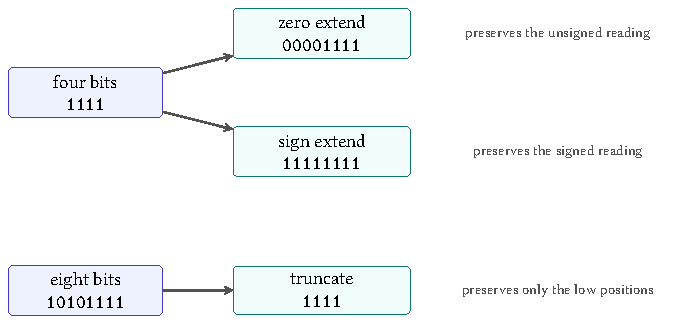
\includegraphics[width=0.86\textwidth]{figures/width-change-map}
\caption{Zero extension, sign extension, and truncation are three different
maps. Their names identify both the bit movement and the reading or positions
they preserve.}
\figalt{The four-bit word 1111 maps to two different eight-bit extensions, while an eight-bit word truncates to its low four positions.}
\label{fig:width-change-map}
\end{figure}

The preservation arguments are short. Zero extension adds only zero
coefficients above the old high bit, so the unsigned sum of bit weights does
not change. For sign extension, a nonnegative source also gains only zeroes.
A negative source of width \(w\), with unsigned representative \(u\), becomes
the wider unsigned representative \(u+2^v-2^w\) at width \(v\). Subtracting
\(2^v\) gives \(u-2^w\), the original signed reading.

This distinction will return in both companion architectures. Their registers
may hold 64-bit words while selected operations produce narrower results.
The semantics must say whether upper bits are preserved, cleared, or supplied
by sign extension.

The words \emph{preserves the value} are incomplete until the reading is
named. Zero extension preserves the unsigned reading. Sign extension
preserves the signed reading. Neither operation promises to preserve both.
For a source whose high bit is zero, they happen to produce the same wider
pattern; that agreement on half the inputs is not a reason to treat the
operations as interchangeable.

\begin{proofkit}[title={\iconProofKit\ Why sign extension preserves a negative value}]
Let a negative width-\(w\) word have unsigned representative \(u\). Its signed
reading is \(u-2^w\). Extending it to width \(v>w\) fills the new high
positions with ones, adding \(2^v-2^w\) to the unsigned representative. The
wider signed reading subtracts \(2^v\):
\[
  \bigl(u+2^v-2^w\bigr)-2^v=u-2^w.
\]
The two large terms cancel, leaving the original signed integer.
\end{proofkit}

Truncation has no such general preservation law. It is a many-to-one map:
every pair of source representatives that differs by a multiple of \(2^v\)
has the same width-\(v\) result. A later proof may still use truncation under a
premise that the discarded bits are known to be zero, or known to repeat the
sign. The premise, not the word \emph{truncate}, earns the preservation claim.

Some compositions do have exact laws. Truncating a zero-extended word back to
its source width returns the original pattern. The same holds after sign
extension because both extensions preserve every original low position.
Extending after truncation does not generally return the original wider word:
the discarded positions are unavailable, so the extension rule must invent
them from zero or from the retained sign bit.

These one-way identities are useful controls. A checker should accept
truncate-after-extend for every source word and reject the reverse identity on
a witness with nonzero discarded positions. The pair teaches more than two
successful examples because it marks exactly where information is lost.

\section{Words and bytes}

A byte is a word of width eight. Memory will store bytes at addresses, so a
wider word needs a declared relation to a sequence of bytes.

\begin{definition}[title={Little-endian split and join}]
Let the word width be a positive multiple of eight. Byte \(i\) is
\[
  b_i =
  \bigl(x \mathbin{\mathrm{div}} 2^{8i}\bigr) \bmod 2^8.
\]
A \keyterm{little-endian} byte sequence puts the lowest-weight byte first in
increasing address order: \(b_0,b_1,\ldots\). Joining the sequence computes
\[
  \sum_i b_i 2^{8i}
\]
at the original width.
\end{definition}

Object \obj{A0.def.byte} records this relation. It does not yet define memory.
It says how one word can be taken apart and put back together.

The reader proof of the round trip is positional. Each \(b_i\) selects exactly
bits \(8i\) through \(8i+7\). Multiplying by \(2^{8i}\) returns those bits to
their original positions. Different bytes occupy \keyterm{disjoint} positions,
meaning that no position belongs to two bytes. Their sum reconstructs the
original word.

For two bytes, write \(x=b_0+2^8b_1\), where both byte values lie between 0
and \(2^8-1\). Splitting extracts \(b_0=x\bmod 2^8\). Dividing \(x\) by
\(2^8\) discards that low remainder and exposes \(b_1\). Joining returns
\(b_0+2^8b_1=x\). For more bytes, the same quotient-and-remainder step repeats.
Nothing in this argument depends on the hexadecimal spelling of \(x\).

\begin{tryit}[title={A byte round trip with unequal digits}]
Split \code{0x00a17c03} into four little-endian bytes. Join them in the proper
order, then join the reversed list. Unequal bytes make an order error visible;
a test word such as \code{0x00000000} would let the wrong rule pass.
\end{tryit}

For \code{0x12345678}, the increasing-address byte sequence is
\code{78}, \code{56}, \code{34}, \code{12}. If we instead attach increasing
addresses to the list \code{12}, \code{34}, \code{56}, \code{78}, the same
little-endian join produces \code{0x78563412}. The numeric word did not
reverse by itself. We changed the relation between addresses and place values.

Width four was useful for the reader proofs because all sixteen cases fit on a
page. A complete A0 state has width equal to a positive multiple of eight.
Here lies the first firm boundary between a proof miniature and the executable
teaching machine.

\section{The two companion questions}

Both later companion slices contain fixed-width integer values and access
byte-addressed memory. That common description does not settle how a given
instruction reads a word, changes its width, or treats its upper bits. Those
rules belong to the selected instruction form.

The question for RV64 and x86-64 is therefore not whether either machine uses
binary. It is which width each form reads, which width it writes, which integer
reading its conditions use, and how its bytes meet memory. We will pin the
exact forms and source revisions before answering those questions as
architectural facts.

The paired questions can now be stated without slogans:

\begin{table}
\centering
\caption{Word-level questions carried from A0 to each real instruction form.}
\begin{tabular}{p{0.21\textwidth}p{0.27\textwidth}p{0.39\textwidth}}
\toprule
Question & RV64 slice & x86-64 slice \\
\midrule
Source width & named operand form & named operand form \\
Destination width & register or memory rule & register, subregister, or memory rule \\
Integer reading & operation and condition & operation and condition \\
Upper bits & explicit width rule & selected subregister rule \\
Byte order & declared memory premise & declared memory premise \\
\bottomrule
\end{tabular}
\end{table}

This table is a checklist, not a set of answers. Saying that one architecture
has 64-bit registers does not settle the result of a narrower write. We need
the exact instruction form and the governing manual revision. Part II will
supply those source-pinned answers after A0 has given us the questions in a
stable order.

\section{The implementation boundary}

The definitions in this chapter are book-level foundations. Axeyum already
has fixed-width bit-vector terms and solver routes, but the redesigned book
does not treat the former width-eight formulas as its word foundation. Object
\obj{OP.a0.word-package} records the actual missing layer: one reusable A0
package for words, readings, width changes, and byte split and join, with
interfaces suitable for execution and proof.

The controls should attack the rules we have just used. A wrong modulus should
fail at wraparound. A wrong sign extension should fail on a source whose high
bit is one. Reversed byte weights should fail on a word with unequal bytes.
A damaged round trip should return a concrete witness rather than a success
message.

An introductory Axeyum workflow will eventually make this obligation
concrete. The reader will construct a fixed-width term, state a relation such
as split followed by join, ask for a counterexample within the declared
width, and replay any returned model through executable A0 operations. If the
solver reports that no counterexample exists, the route must still identify
the generated formula and the independent checking boundary. Axeyum's current
bit-vector machinery is useful substrate for that route; it is not yet the A0
word package named by this chapter.

The first Python-facing lesson should use a small, typed surface. Construct a
word by giving its width and natural representative. Ask for its unsigned and
signed readings. Apply one width change or byte split. The bound Rust type
should reject a value outside the constructor contract rather than silently
choosing a width. Python may format binary and hexadecimal views, but Rust
must own the carrier and operations that later checks reuse.

The proof-facing lesson begins from the same objects. It quantifies over a
declared width, applies the executable operation or its matched formula
encoding, and requests either a separating input or evidence that the finite
claim has no separating input. Replaying a returned word must reproduce both
its stored pattern and the observations that made it a counterexample.

This progression keeps three activities distinct: calculating one example,
searching the whole finite domain, and checking the evidence returned by that
search. The commands may be close together in a notebook. Their claims are
not interchangeable.

\begin{sidebar}[title={What Axeyum will add}]
The mathematics on these pages defines the intended word operations. The
planned Axeyum package will add executable operations, formula generation,
counterexample replay, checked evidence for selected finite claims, and
negative controls. It will not turn an unstated width convention into a
theorem.
\end{sidebar}

Until that package exists, this chapter has reader proofs and exact
definitions but no generated machine-proof box. A solver result about one
handwritten formula would not establish the width-parametric library on which
later A0 state and instruction semantics must depend.

One word now has a carrier, bit operations, several readings, width changes,
and a relation to bytes. It still has no location. We do not know which
register holds it, which memory address names one of its bytes, which
instruction comes next, or whether execution has stopped. Chapter 2 constructs
the state in which those questions have answers.

\section{Exercises}

\begin{enumerate}
\item \textbf{Execute.} Compute every width-four sum \(x+1\). Explain the wraparound once by
enumeration and once by the remainder definition.
\item Find two width-four additions with the same stored result but different
signed or unsigned interpretations.
\item Convert \code{0x9d} to eight binary digits. Use masks and shifts to
extract its low three bits and its high three bits.
\item Zero-extend and sign-extend each width-four pattern whose high bit is
one. State which integer reading each operation preserves.
\item For every pair among \code{0111}, \code{1111}, and \code{0001}, compute
the width-four sum, unsigned carry out, and signed overflow. Explain each
disagreement between the two conditions.
\item \textbf{Transfer.} Split \code{0x89abcdef} into little-endian bytes and join them again.
Then reverse the byte list and calculate the different word it represents.
\item \textbf{Prove.} Prove that splitting and joining a two-byte word returns the original
word. Identify the exact step that generalizes to any positive byte count.
\item \textbf{Break.} Design a false join rule by changing one exponent. Give a word whose
round trip exposes the error. This will become the negative control for the
future A0 word package.
\item \textbf{Prove.} Show that bitwise exclusive or with a fixed mask is its
own inverse. State why the argument works independently at every bit position.
\item \textbf{Break.} Give a pair of different width-eight words that truncate
to the same width-four word. Then state a premise under which truncation would
preserve the unsigned reading.
\end{enumerate}
